\documentclass[internal]{nhitec_design}

\usepackage{listings}

\author{ROTHEUDT Thomas et MOUCHAMPS Antoine}
\date{\today}

\title{Installation de Laravel \& Docker}

\newRem{tom}{green!60!black}

\begin{document}

\maketitle
\newpage
{
\hypersetup{linkcolor=black}
\color{red_nhitec}
\tableofcontents
}

\newpage

\section[Introduction]{Introduction}
    \subsection[Qu'est-ce que Docker?]{Qu'est-ce que \docker{}?}
        
        \docker{} est un outil open-source créé en 2012 par des français. Cet outil permet de créer, de déployer et de lancer des applications tournant dans un conteneur. Ces conteneurs sont en réalité des environnements dans lesquels les applications tournent.
        Ils sont créés grâce à des images qui sont des fichiers \docker{}, ainsi n'importe quel conteneur est assuré de tourner sur n'importe quel machine sans se soucier des configurations locales.\\
        L'outil est tellement populaire que les mainteneurs de librairies ou de logiciels maintiennent des images \docker{} (dans notre cas on verra que \laravelsail{} possède une image \docker{} qui est maintenue à jour régulièrement)
        Il permet donc de ``centraliser'' l'environment sur lequel une application est développée. 

        \begin{figure}[h]
            \centering
            \begin{subfigure}[b]{0.3\textwidth}
                
\includegraphics[scale=0.4]{Images_formation/LogoDocker.pdf}
            \end{subfigure}%
        \end{figure}
        
    \subsection[Pourquoi Docker?]{Pourquoi \docker{}?}

        Un conteneur \docker{} possède de nombreux avantages comparé aux machines virtuels. Premièrement, il utilise les ressources d'un système plus éfficacement qu'une VM tout en gardant ses avantages (isolation et reproductibilité). 

        \begin{wrapfigure}{l}{0.18\textheight}
            \centering
            
\includegraphics[width=0.2\textwidth]{Images_formation/Iconconteneur.pdf}
        \end{wrapfigure}

        Il garanti d'être identique quel que soit le système, ainsi chaque membres d'un projet est certain de travailler sur le même environment sans se soucier de la portabilité de l'application sur l'environment final.
        
        Les conteneurs sont isolés de la machine hôte, ainsi vous pouvez avoir plusieurs versions différentes de dépendances pour plusieurs projets.

        Enfin, la modifications d'un conteneurs est extrêmement simplifié comparé à une VM où les mises à jour sont souvent complexes et laborieuse.

        Pour résumer, un conteneur \docker{} est flexible, léger, portable.

        
\newpage

    \subsection[Qu'est-ce que Laravel Sail?]{Qu'est-ce que \laravelsail{}?}
        
        \laravelsail{} est une interface de ligne de commande légère pour interagir avec l'environnement de développement \docker{} par défaut de \laravel{}. 
        
        \begin{wrapfigure}{l}{0.2\textwidth}
            \centering
            
\includegraphics[width=0.2\textwidth]{Images_formation/LaravelLogo.pdf}
        \end{wrapfigure}
        
        Sail est un excellent point de départ pour construire une application \laravel{} en utilisant \php{}, \mysql et Redis sans avoir besoin d'une expérience préalable de \docker{}.

        Au cœur de Sail se trouve le fichier docker-compose.yml et le script sail qui est stocké à la racine de votre projet. Le script sail fournit une CLI (command line interface) avec des méthodes pratiques pour interagir avec les conteneurs \docker{} définis par le fichier docker-compose.yml.

        \laravelsail{} est pris en charge sur \macos{}, \linux{} et \windows{} (via WSL2).

        Pour résumer, le scrip sail permet de gérer le projet \laravel{} à l'intérieur du conteneur du projet. De plus \laravelsail{} est complètement compatible avec \docker{}, ce qui permet des interactions plus simples avec les conteneurs.

\section[Installation de Docker]{Installation de Docker 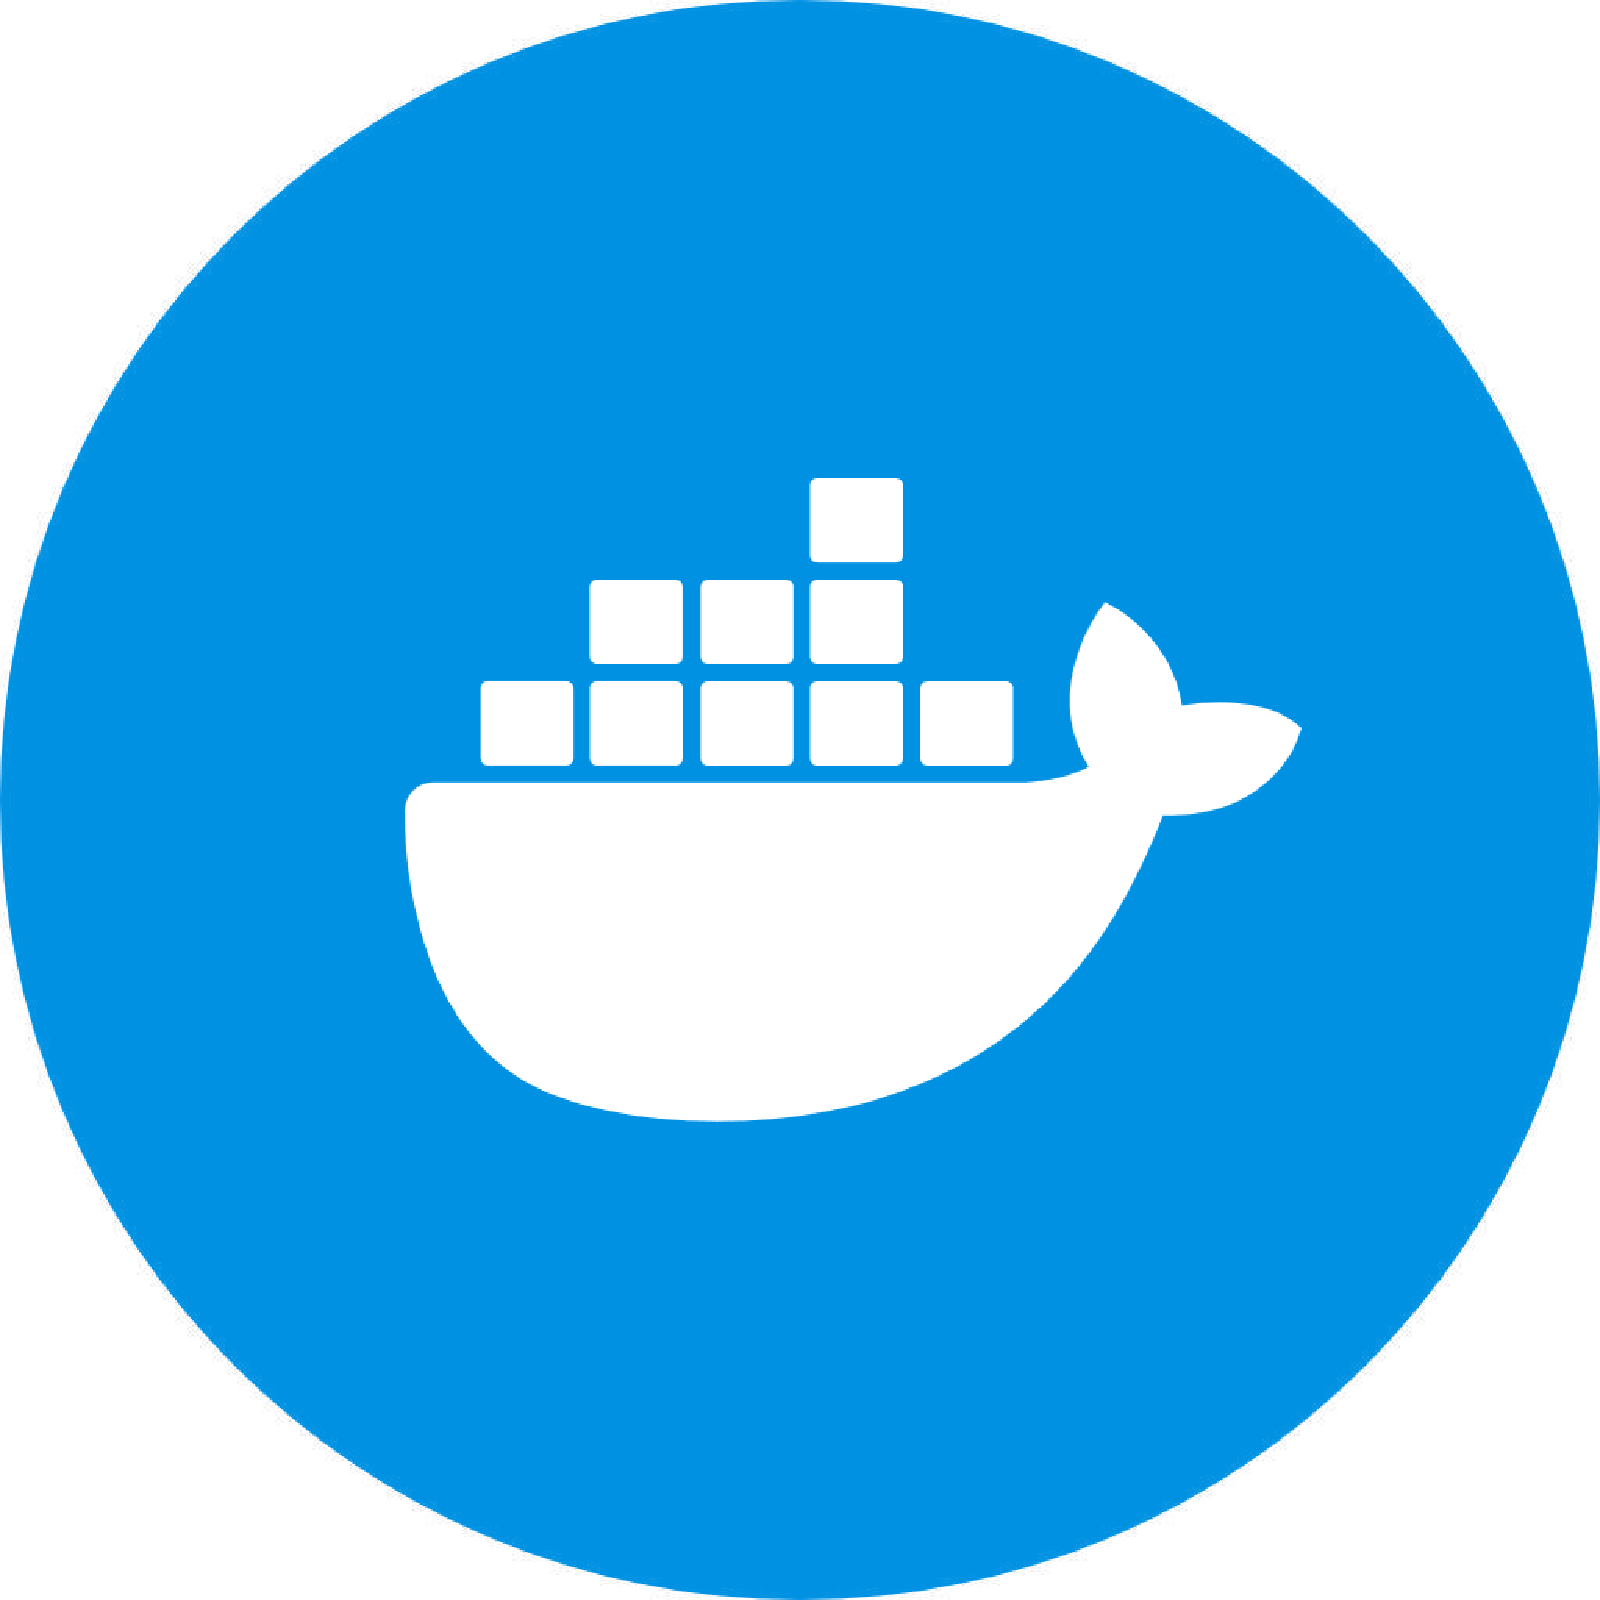
\includegraphics[height=15pt]{figures-logos/docker.pdf}}

Choisissez la section correspondant à votre système d'exploitation:

\begin{figure}[!h]
    \centering
    \begin{minipage}{0.32\textwidth}
        \centering
        
\includegraphics[scale=0.05]{Images_formation/LinuxLogo.pdf}
        \caption*{\underline{Linux}: \textsc{section~\ref{sec:installation_linux}}}
    \end{minipage} 
    \begin{minipage}{0.32\textwidth}
        \centering
        
\includegraphics[scale=0.025]{Images_formation/WindowsLogo.pdf}
        \caption*{\underline{Windows}: \textsc{section~\ref{sec:installation_windows}}}
    \end{minipage}
    \begin{minipage}{0.32\textwidth}
        \centering
        
        
\includegraphics[scale=0.025]{Images_formation/MacosLogo.pdf}
        \caption*{\underline{MacOS}: \textsc{section~\ref{sec:installation_macos}}}
    \end{minipage}
\end{figure}

    \subsection[Installation Linux]{Installation \linux{}\label{sec:installation_linux}}

        L'Installation \linux{} nécéssite de suivre quelques étapes de plus que pour l'Installation \macos{} ou \windows{}.\\
        \begin{itemize}
     
            \item[1.] Mettez à jour l'index des paquets apt et des paquets d'installation pour permettre à apt d'utiliser un dépôt sur HTTPS:
            
                \begin{lstlisting}
                    sudo apt-get update
                \end{lstlisting}

            \item[2.] Installez les dépendances de \docker{}:

                \begin{lstlisting}
                    sudo apt-get install \
                        ca-certificates \
                        curl \
                        gnupg \
                        lsb-release
                \end{lstlisting}

            \item[3.] Ajoutez la clé GPG officielle de \docker{}:

                \begin{lstlisting}
                    sudo mkdir -m 0755 -p /etc/apt/keyrings

                    curl -fsSL https://download.docker.com/linux/ubuntu/gpg | 
                    sudo gpg --dearmor -o /etc/apt/keyrings/docker.gpg
                \end{lstlisting}

            \item[4.] Configurez le répertoire:\\

                \begin{footnotesize}
                    \textit{\textdollar(lsb\_release -cs)} doit dans quelques cas être remplacé par votre version de distribution \linux{}.\\
                    Dans l'installation de référence on a remplacé par \textit{jammy}.
                \end{footnotesize}
                \begin{lstlisting}
                    echo \
                    "deb [arch=\$(dpkg --print-architecture) 
                    signed-by=/etc/apt/keyrings/docker.gpg] https://download.docker.com/linux/ubuntu \
                    \$(lsb_release -cs) stable" 
                    | sudo tee /etc/apt/sources.list.d/docker.list > /dev/null
                \end{lstlisting}

            \item[5.] Verifiez que le répertoire est bien configurer:

                \begin{lstlisting}
                    sudo apt-get update
                \end{lstlisting}    

            \item[6.] Installez Docker Engine, conteneurd, et Docker Compose:

                \begin{lstlisting}
                    sudo apt-get install docker-ce docker-ce-cli 
                    conteneurd.io docker-buildx-plugin docker-compose-plugin
                \end{lstlisting}
                \begin{footnotesize}
                    Vous pouvez tester votre installation avec la commande: \textit{sudo docker run hello-world}
                \end{footnotesize}

                \bigskip
            \item[7.] Installez \dockerdesktop{}:

            
                \begin{footnotesize}
                    Téléchargez le \href{https://desktop.docker.com/linux/main/amd64/docker-desktop-4.17.0-amd64.deb?utm_source=docker&utm_medium=webreferral&utm_campaign=docs-driven-download-linux-amd64}{Docker Destop} et l'installez avec la commande:
                \end{footnotesize}

                \begin{lstlisting}
                    sudo apt-get install ./docker-desktop-<version>-<arch>.deb
                \end{lstlisting}

        \end{itemize}

\bigskip

        \begin{footnotesize}
            L'Installation de référence pour ce guide a été faite sur une distribution \linux{} Mint (distibution basé sur \ubuntu{})\\
        \end{footnotesize}

        \hyperref[sec:suite]{Pour passer à la suite}

\newpage

    \subsection[Installation Windows]{Installation \windows{}\label{sec:installation_windows}}

        \subsubsection[Prérequis][fr.wikipedia.org/wiki/Windows_Subsystem_for_Linux]{Prérequis: WSL2}

        Pour utiliser \dockerdesktop, il est fortement conseillé d'utiliser \href{https://learn.microsoft.com/fr-fr/windows/wsl/install}{WSL2}. C'est une application \windows{} permettant d'installer un environnement \linux{} avec la distribution de votre choix nativement sous \windows{}. 

        Pour l'installer, il suffit de lancer \verb|wsl --install| dans le terminal de \windows{} de base ou \texttt{Powershell}\footnote{Attention, le terminal choisi doit être exécuté en tant qu'administrateur !}. Par défaut, cette commande installera \ubuntu{} comme système \linux. Pour d'avantage d'informations conçernant l'installation de WSL2, consultez le lien vers la page officielle de Microsoft. Si tout se passe bien vous devriez recevoir le message suivant:

        \begin{figure}[!th]
            \centering
            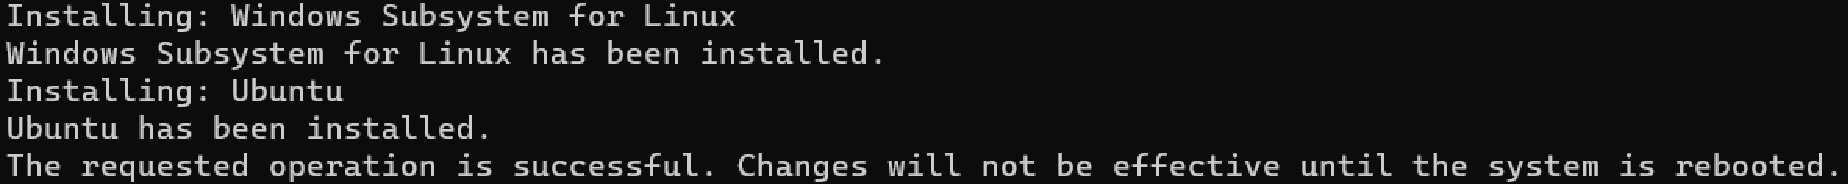
\includegraphics[width=0.75\textwidth]{Images_formation/ubuntu_installation.pdf}
        \end{figure}

        Après avoir redémarer votre PC, la fenêtre suivante devrait apparaitre. Si ce n'est pas le cas, chercher \texttt{wsl.exe} dans la barre de recherche windows et lancez le terminal.

        \begin{figure}[!th]
            \centering
            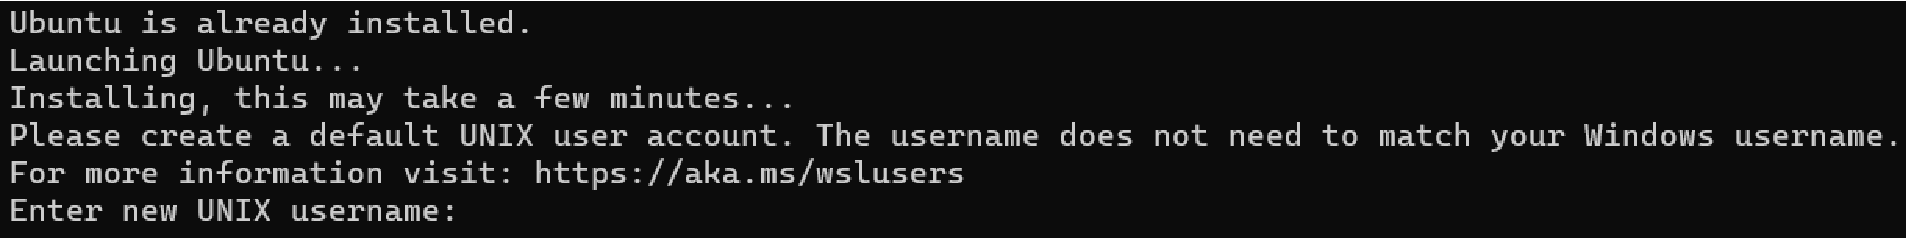
\includegraphics[width=0.75\textwidth]{Images_formation/user_creation.pdf}
        \end{figure}

        Ici, vous devez créer un utilisateur ainsi qu'ajouter un mot de passe\footnote{Lorsque vous tapez votre mot de passe, il est normal que les charactères ne s'affichent pas.}

        Une fois ces étapes effectuées sans accros, vous pouvez passer à l'installation de \dockerdesktop à proprement parlé.

        \subsubsection[Installation de Docker Desktop]{Installation de \dockerdesktop}
        
        \begin{itemize}
            \item[1.] Téléchargez \href{https://desktop.docker.com/win/main/amd64/Docker%20Desktop%20Installer.exe}{\dockerdesktop{}}
            
            \item[2.] Exécutez le fichier d'installation \verb|.exe|
            
            \item[3.] Vérifiez l'installation en lançant votre environment \verb|wsl| et en tapant la commande suivante:
            \begin{lstlisting}
                docker
            \end{lstlisting}
        \end{itemize}

        \docker{} et wsl2 sont totalement compatibles. C'est pourquoi vous devez cocher l'option ``use WSL2'' pendant l'installation. 

        \hyperref[sec:suite]{Pour passer à la suite}

    \newpage
    \subsection[Installation MacOS]{Installation \macos{}\label{sec:installation_macos}}

        \begin{itemize}
            \item[1.] Téléchargez \dockerdesktop{} \href{https://desktop.docker.com/mac/main/arm64/Docker.dmg?utm_source=docker&utm_medium=webreferral&utm_campaign=dd-smartbutton&utm_location=module}{Apple Chip} ou \href{https://desktop.docker.com/mac/main/amd64/Docker.dmg?utm_source=docker&utm_medium=webreferral&utm_campaign=dd-smartbutton&utm_location=module}{Intel Chip}
            \item[2.] Installez \dockerdesktop{} dans le dossier application
        \end{itemize}

        \hyperref[sec:suite]{Pour passer à la suite}

\newpage

    \subsection[Aperçu]{Aperçu\label{sec:suite}}

        Si tout s'est bien passé vous êtes en mesure de lancer \dockerdesktop{}. 
        Vous avez donc le panneau de contrôle de \dockerdesktop{} qui devrait ressembler à ça:\\
        
        \begin{figure}[h]
            \centering
            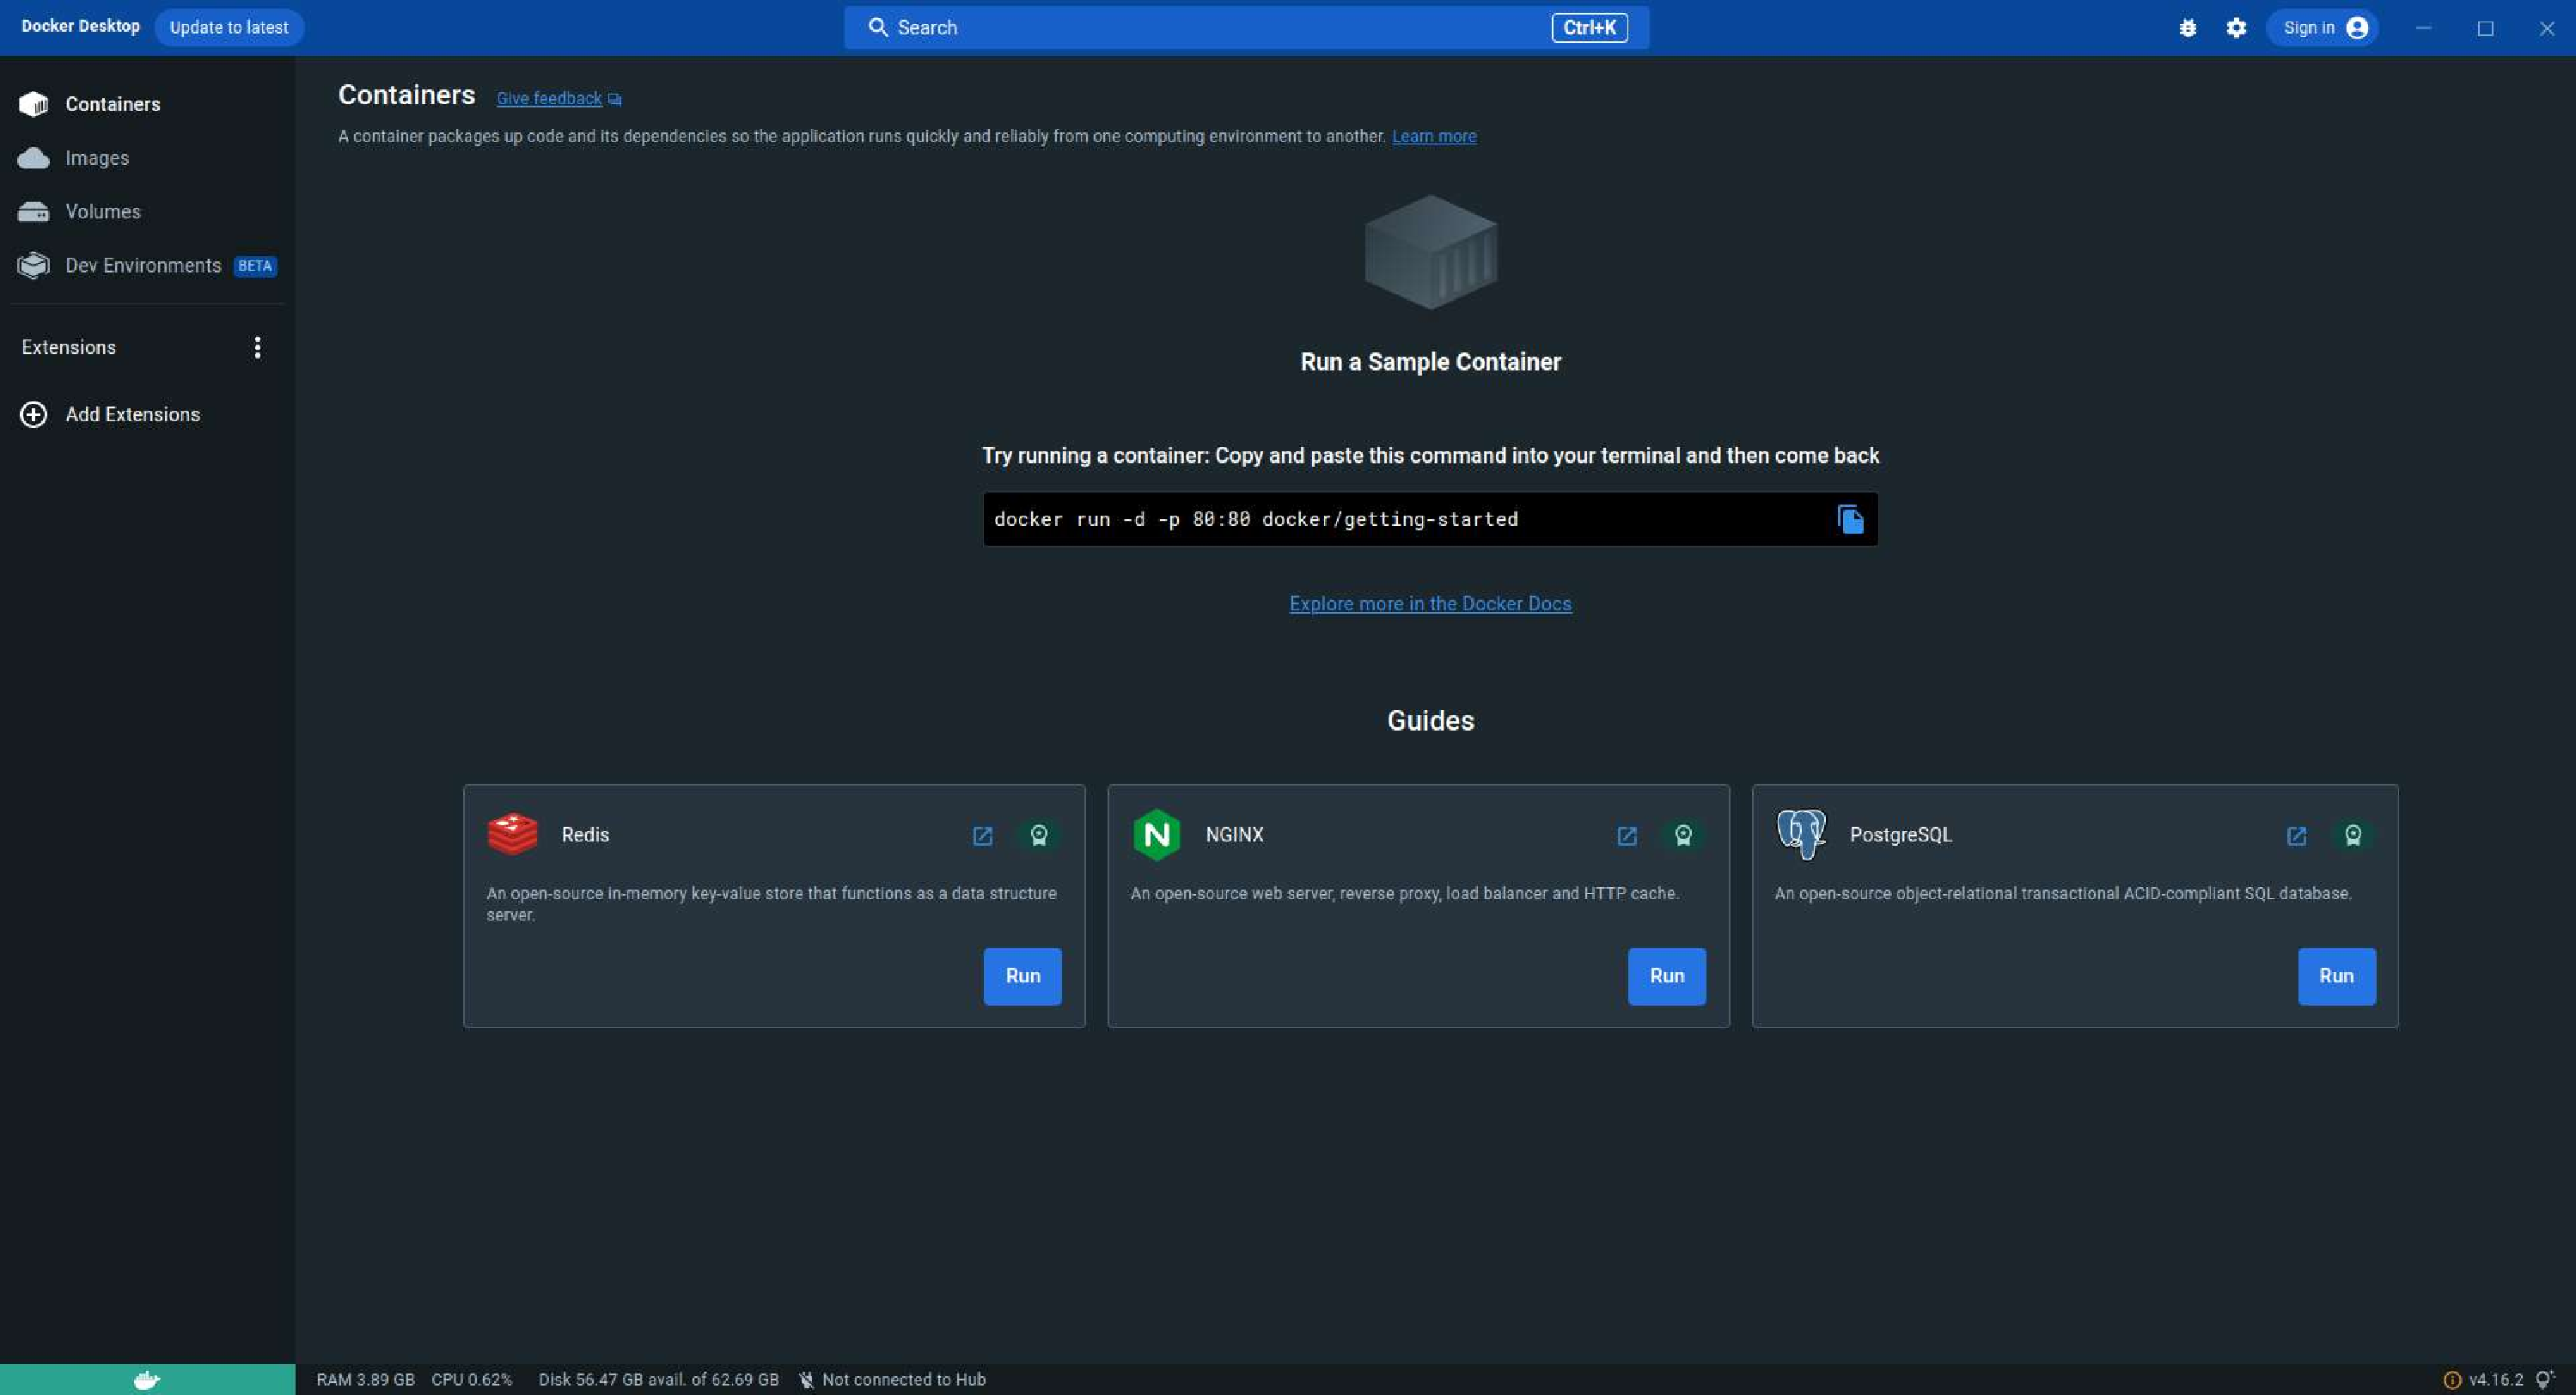
\includegraphics[scale=0.25]{Images_formation/PanelDocker.pdf}
        \end{figure}

        Vous pouvez voir différents onglets sur la gauche:

        \begin{itemize}
            \item Conteneurs: Cet onglet va contenir tous les conteneurs que vous avez créés. Les conteneurs sont en quelque sorte des images déployées et exécutées lorsque \docker{} tourne.\vspace*{0.5cm}
            \item Images: Cet onglet va contenir toutes les images d'installation des services installés dans nos conteneurs. Les images décrivent l'environnement du serveur, les packages installés et toutes les configurationde celui-ci.\vspace*{0.5cm}
            \item Volumes: Cet onglet contient les volumes liés aux services qui contiennent les data de nos applications. Les volumes servent à conserver les données des \db lorsque nous éteignons un container et qu'on le relance.\vspace*{0.5cm}
            \item Dev Environnements: une feature très intéressante permettant de créer des environnements de développement \footnotesize{\href{https://docs.docker.com/desktop/dev-environments/}{(plus d'informations)}}.
        \end{itemize}

    \subsection[VS Code]{Utilisez \vscode!!}
    Enfin, pour utiliser tout ce que nous venons d'installer, il faut un éditeur de code efficace. \href{https://code.visualstudio.com/}{\vscode{}} permet, via ses extensions d'interagir avec \docker{} et WSL2 en parfaite harmonie, c'est pourquoi nous le recommandons CHAUDEMENT. 

    Une fois \vscode{} installez, ajouter les extensions WSL (de Microsoft) et Docker (de Microsoft également).





\newpage
\section[Création Projet Laravel]{Création Projet \laravel{}}

    \subsection{Création du dossier}
        Pour créer un nouveau projet \laravel{} dans un dossier ``exemple-app'' il suffit juste d'entrer la ligne de commande:

        \begin{lstlisting}
            curl -s https://laravel.build/example-app | bash
        \end{lstlisting}

        Avec cette commande votre projet sera installé avec plusieurs services de base (mysql, redis, et d'autres)

        il est possible de choisir les services à installer avec le mot clé \textit{with}

        \begin{lstlisting}
            curl -s "https://laravel.build/example-app?with=mysql,redis" | bash
        \end{lstlisting}
        Mais pour plus de claireté, on va utiliser la première commande.

        une fois lancé le projet va se créer (cela peut prendre un certain temps)

        \begin{figure}[h]
            \centering
            \begin{subfigure}{0.3\textwidth}
                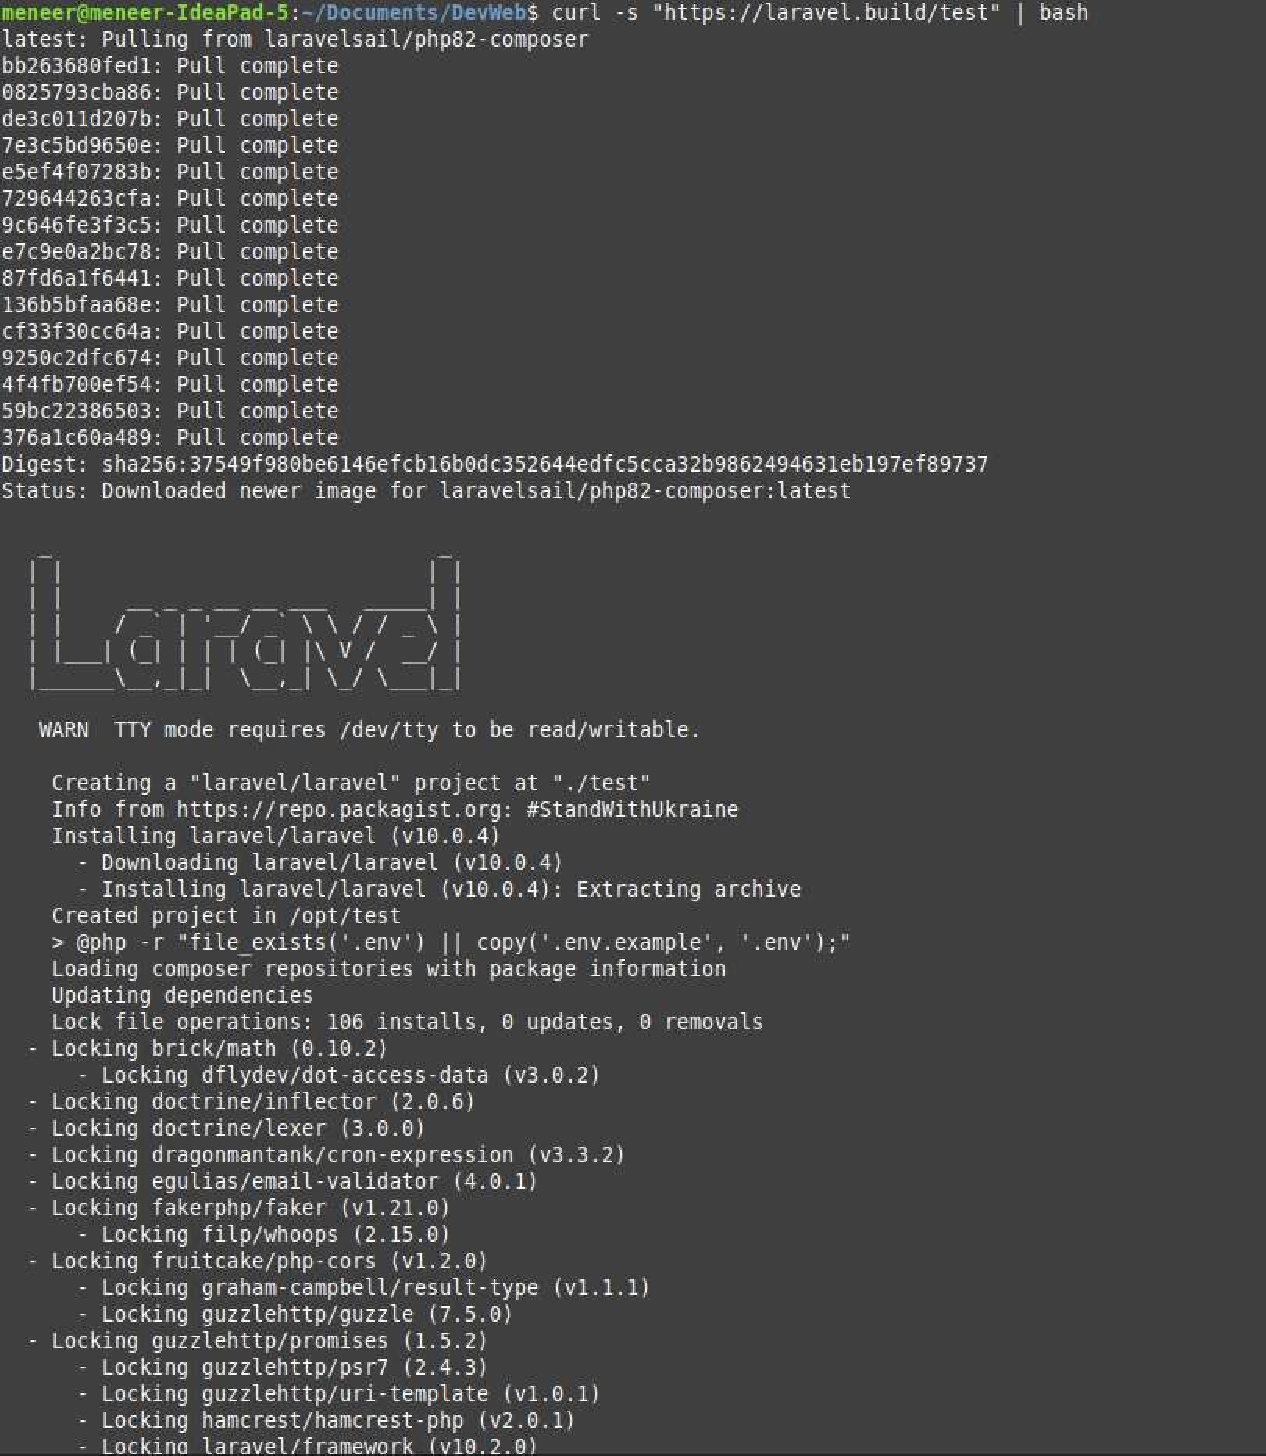
\includegraphics[width=\textwidth]{Images_formation/CreateProject.pdf}
            \end{subfigure}
            \begin{subfigure}{0.3\textwidth}
                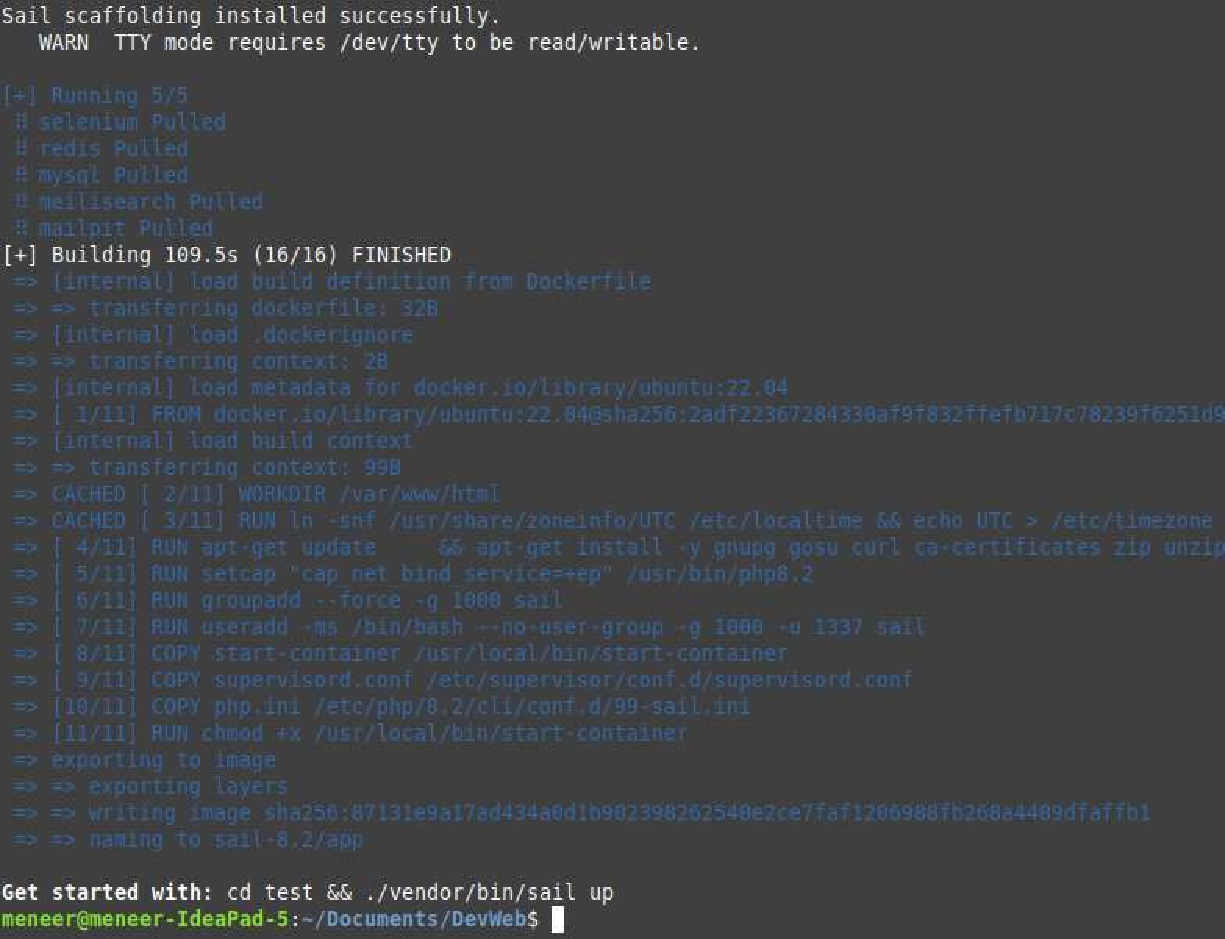
\includegraphics[width=\textwidth]{Images_formation/CreateProject2.pdf}
            \end{subfigure}
        \end{figure}


        Une fois le dossier du projet créé vous allez rentrer dans le Dossier et ouvrir le fichier \textit{docker-compose.yml}.

        Ce fichier représente la configuration générale de votre conteneur, c'est ici que l'on va définir les services à installer, les versions, les images, ect.
        Ce fichier est très important, sans lui, pas de conteneur.

        Vous pouvez voir qu'il est composé de plusieurs \href{https://docs.docker.com/compose/compose-file/}{section}, \textit{Version, services, network, volumes}. Chaque section à son utilitée. Nous allons nous concentrer sur la section service du fichier. Plus précisement, nous allons ajouter un service.\\ 


\newpage

    \subsection[Ajout PhpMyAdmin]{Ajout \phpmyadmin{}}

        On va ajouter un service à notre projet qui est nécessaire à la gestion de notre base de donnée,\\ \phpmyadmin{}.
        
        Pour ce faire, rendez-vous à la fin de la section \verb|services|, et ajoutez y \phpmyadmin{} comme suit:

        \begin{lstlisting}
            phpmyadmin:
                image: 'phpmyadmin:latest' 
                ports:
                    - '8080:80' 
                networks:
                    - sail 
                environment:
                    - PMA_ARBITRARY=1
        \end{lstlisting}

        Une fois cela fait, \phpmyadmin{} est intégré au projet.

    \section[Utilisation]{Utilisation}
    Pour utiliser le script, il vous faudra utiliser la commande suivante dans le dossier du projet (sail est installé par defaut lors de la création du projet):

    \begin{lstlisting}
        ./vendor/bin/sail [command] [options] [arguments]
    \end{lstlisting}

    Vous pouvez créer un alias pour sail en ajoutant la ligne suivante à votre .bashrc, zshrc, ect: 

    \begin{lstlisting}
        alias sail='[ -f sail ] && sh sail || sh vendor/bin/sail'
    \end{lstlisting}
    
    \subsection[Démarrage du container]{Démarrage du container}
        Pour lancer le container et ainsi pouvoir travailler sur le projet, entrez dans le dossier de votre projet via un terminal et lancer la commande:
        
        \begin{lstlisting}
            sail up -d
        \end{lstlisting}

        Cette commande lancera le container en mode détacher pour garder l'accès au terminal (pratique si l'on travaille sur VSCode)\\
        \footnotesize{On peut aussi lancer dans un terminal avec \textit{sail up}}


        Vous pouvez maintenant avoir accès à la page de votre projet en allant sur \textit{localhost} via un moteur de recherche comme Mozilla, Google, ect.

    \subsection{Arrêt du container}

    Pour éteintre le container lorsque vous avez finis de travailler, tapez la commande

    \begin{lstlisting}
        sail down
    \end{lstlisting}
    \end{document}
